\section{Introduction} 
\label{Plots}

This is our explanation of why the LHC experiments produce summary plots for example scenarios, breathtaking in its clarity and brevity.

\begin{figure}[h!]
    \centering
	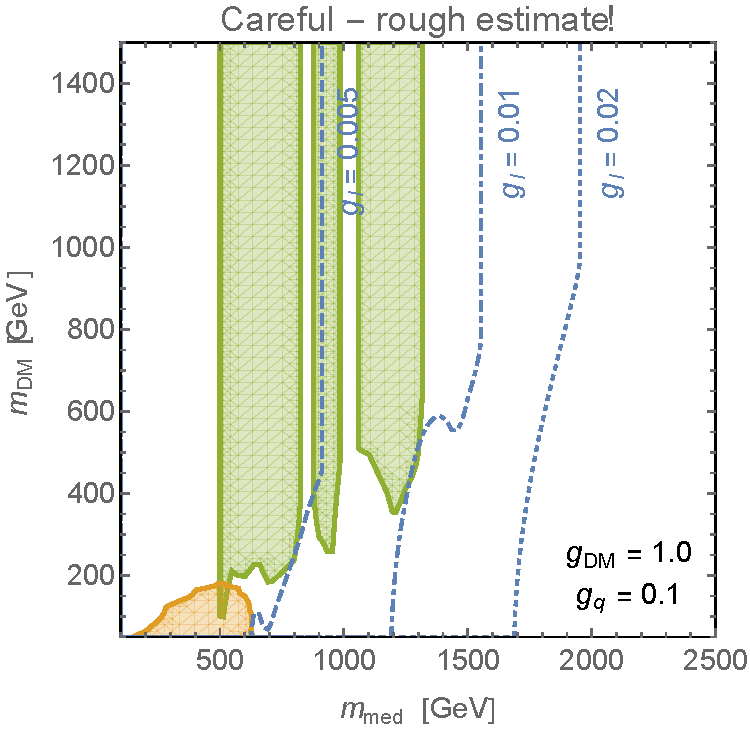
\includegraphics[width=0.5\textwidth]{figures/mass-mass.pdf}
  \caption{This is a sample figure.}
    	\label{fig:DMComplementarity}
\end{figure}

Do we address whether or not to map dijet and dilepton constraints to the direct detection cross section plots, as we do for the mono-X results?
